 \documentclass{beamer}

\usepackage{ucs}
\usepackage[utf8x]{inputenc}
\usepackage[T1]{fontenc}
\usepackage[english]{babel}
\usepackage[retainorgcmds]{IEEEtrantools}%	IEEEeqnarray
\usepackage{mathabx}%	convolution symbol
\usepackage{multi row}
\usepackage{epstopdf}
\usepackage{listings}
\lstset{
	language=c,
	basicstyle=\footnotesize,
	showtabs=true,
	tabsize=3,
}

%	presentation info
\title{Study and Optimization of a Finite Volume's Method Application}

\author{José Alves, Rui Brito}

\institute[pg22765, pg22781]{
	Universidade do Minho
}

\date{Braga, November 2012}


%	beamer options
\usetheme{Frankfurt}


\begin{document}%	begin presentation

\maketitle%	title slide

\begin{frame}
	\frametitle{Index}
	\tableofcontents
\end{frame}

\section{Case Study}

\begin{frame}[plain]
	\frametitle{Convexion-Diffusion}
	\begin{description}
		\item [What?] Calculates the heat diffusion of a fluid while it spreads through an area;
		\item [How?] Uses finite-volumes method;
		\item [Why?] Represents surface as a mesh, making each cell only dependent of its neighbours;
	\end{description}
\end{frame}

\begin{frame}[plain]
	\frametitle{Convexion-Diffusion}
	\begin{description}
		\item [makeFlux] Compute the contribution from each edge;
		\item [makeResidual] Compute the $\phi$ vector, adding the flux for each cell from each contribution;
		\item [LUFactorize] Calculate the matrix form of a Gauss elimination;
	\end{description}
\end{frame}


\section{Test Methodology}

\begin{frame}[plain]
	\frametitle{Test Machines}
		\begin{center}

			\begin{table}[!htp]
			\resizebox{\textwidth}{!}{
			\begin{tabular}{|c|c|c|c|}
			\hline
			 & compute-511-2@search & compute-611-1@search & MacBookPro\\
			 & AMD Opt 6174 & Xeon X5650 & Intel Ivy-Bridge i7\\
			\hline
			\# processors & 2 & 2 & 1\\
			\# cores per processor & 12 & 6 & 4\\
			hyper-threading & - & yes & yes\\
			clock frequency(GHz) & 2.2 & 2.66 & 2.3\\
			L1 capacity & 128KB & 128KB & 64KB\\
			L2 capacity & 512KB & 256KB & 256KB\\
			L3 capacity & 12MB & 12MB & 6MB\\
			RAM capacity & 64GB & 48GB & 16GB\\
			\hline
			\end{tabular}}
			\caption{Test machines}
			\label{tab:test machines}
			\end{table}
		\end{center}
\end{frame}

\begin{frame}[plain]
	\frametitle{Test Parameters}
	\begin{description}
		\item [-] Best of 3 executions within a 5\% error margin of each other;
		\item [-] Test for different number of threads across various systems;
		\item [-] Single user mode;
	\end{description}
\end{frame}


\section{Sequential version}

\begin{frame}
	\frametitle{Original version}
	\begin{description}
	\item [-] For each edge:
	\begin{description}
		\item [-] Calculate edge velocity;
		\item [-] Calculate flux;
	\end{description}
	\item [-] For each cell:
	\begin{description}
		\item [-] Compute all contributions;
	\end{description}
	\item [-] Compute vector $\phi$;
	\item [-] Compute the matrix form of a Gauss elimination;
	\item [-] Compute the error;
	\end{description}
\end{frame}

\begin{frame}
	\frametitle{Challenges}
	\begin{description}
	\item [-] High number of memory accesses;
	\item [-] Low operational intensity;
	\item [-] Deep memory indirection chain;
	\end{description}
\end{frame}

\begin{frame}
	\frametitle{Optimized version}
	\begin{description}
		\item [-] Removed redundant loads and calculations;
		\item [-] Changed some variable definitions to \emph{const};
		\item [-] Usage of a recent compiler(SLP);
		\item [-] Reduced makeResidual's workload from 9.2\% to 5.53\%;
		\item [-] Improved computation time from 12.47s to 8.29s;
	\end{description} 
\end{frame}

\section{PAPI Analysis}

\begin{frame}
	\frametitle{Counters Used}
	\begin{description}
		\item[PAPI\_TOT\_INS] Total instructions;
		\item[PAPI\_LD\_INS] Load Instructions;
		\item[PAPI\_SR\_INS] Store Instructions;
		\item[PAPI\_FP\_OPS] Floating point operations;
		\item[PAPI\_L1\_DCA] L1 data cache accesses;
		\item[PAPI\_L2\_DCA] L2 data cache accesses;
	\end{description}
\end{frame}

\begin{frame}
	\frametitle{PAPI comparison}
	\begin{center}

			\begin{table}[!htp]
			\resizebox{\textwidth}{!}{
			\begin{tabular}{|c|c|c|}
			\hline
			 & original version & optimized sequential version\\
			\hline
			Total instructions & 2.517.584 & 285.551\\
			Load instructions & 630.156 & 86.532\\
			Store instructions & 326.459 & 39.208\\
			FP operations & 55.673 & 44.019\\
			L1 data accesses & 1.061.761 & 153.593\\
			L2 data accesses & 22.914 & 17.467\\
			\hline
			\end{tabular}}
			\caption{PAPI comparison}
			\label{tab:testcases}
			\end{table}
		\end{center}

\end{frame}


\section{OpenMP Implementation}

\begin{frame}
	\frametitle{OpenMP Objectives}
	\begin{description}
		\item [-] Parallelize application;
		\item [-] Decrease runtime;
	\end{description}
\end{frame}	


\begin{frame}
	\frametitle{Amdahl's Law}
		\begin{center}
		$S_{N}=\frac{1}{(1-P) + P/N}$

		
			\begin{table}[!htp]
			\begin{tabular}{|r|r|r|}
			\hline
			\textbf{Parallel Portion} & \textbf{\# Cores} & \textbf{Expected Speedup}\\
			\hline
			 & 1 & 1 \\
			 & 2 & 1.0284 \\
			 & 4 & 1.0433 \\
			 5.53\% & 8 & 1.0508 \\
			 & 12 & 1.0534 \\
			 & 16 & 1.0547 \\
			 & 24 & 1.0560 \\
			\hline
			\end{tabular}
			\caption{Theoretical speedups}
			\label{tab:testcases}
			\end{table}
		\end{center}	
\end{frame}

\begin{frame}
	\frametitle{Achieved Results}
	\begin{center}

	\begin{figure}[!htp]
		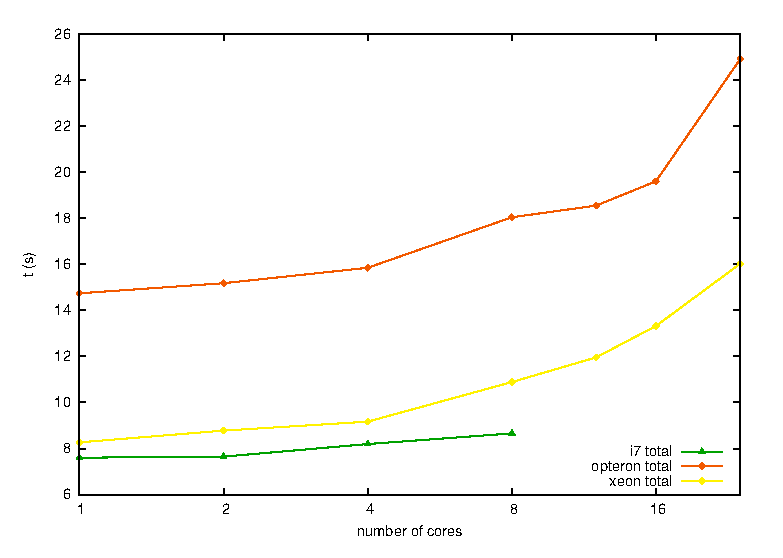
\includegraphics[width=10cm]{images/total.eps}
		\caption{Total application runtime}
		\label{fig:roofline}
	\end{figure}
	\end{center}
\end{frame}

\begin{frame}
	\frametitle{Achieved Results}
	\begin{center}

	\begin{figure}[!htp]
		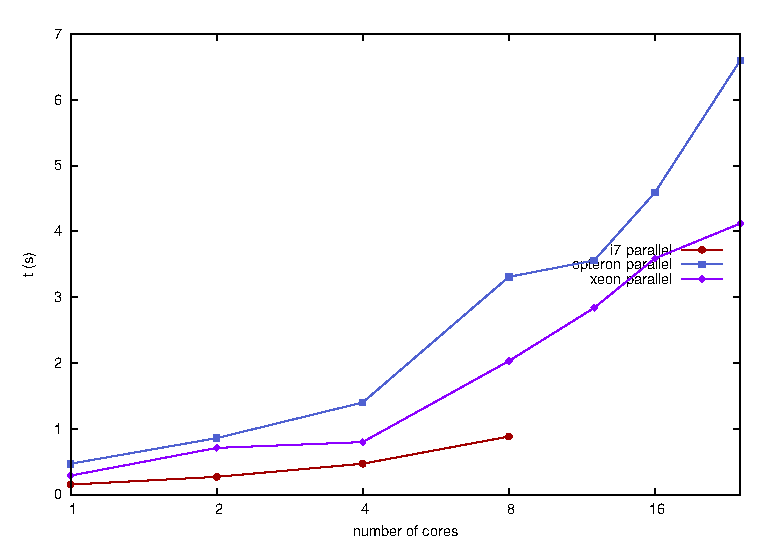
\includegraphics[width=10cm]{images/parallel.eps}
		\caption{Parallel section runtime}
		\label{fig:roofline}
	\end{figure}
	\end{center}
\end{frame}


\section{On-going and future work}
\begin{frame}
	\begin{center}
	\begin{itemize}
		\item GPU version delayed;
		\item Thorough restructuring of the code;
		\item FVLib optimizations;
		\item Improve IO;
		\item MPI version;
	\end{itemize}
	\end{center}
\end{frame}

\section{Questions}
\begin{frame}
	\titlepage
	
	
\end{frame}

\end{document}%	end presentation